\documentclass[border=3pt,tikz]{standalone}
\usepackage[utf8]{vietnam}
\usetikzlibrary{calc,angles,intersections,shapes.geometric,arrows,decorations.markings,arrows.meta,patterns.meta,patterns}
\usepackage{tikz-3dplot,pgfplots}
\pgfplotsset{compat=1.15}
\usepgfplotslibrary{polar}
\usepackage{amsmath}
\begin{document}
	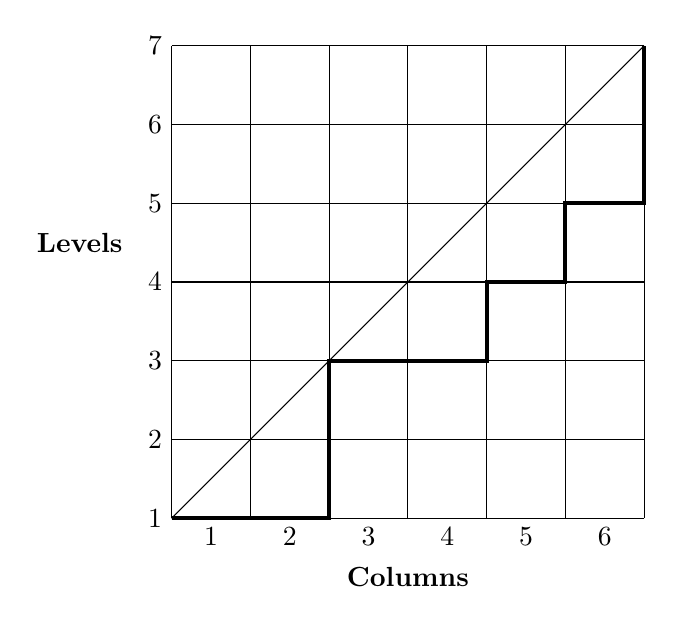
\begin{tikzpicture}
		\foreach \i in {0,...,6}{\draw (\i,0)--(\i,6) (0,\i)--(6,\i);}
		\foreach \i in {1,...,6}{\draw (\i-0.5,0)node[below]{$\i$} (0,\i-1) node[left]{$\i$};}
		\draw (0,6)node[left]{$7$};
		\draw (0,0)--(6,6);
		\draw[line width=1.5] (0,0)--(2,0)--(2,2)--(4,2)--(4,3)--(5,3)--(5,4)--(6,4)--(6,6);
		\draw (-0.5,3.5) node[left]{\bf Levels} (3,-0.5) node[below]{\bf Columns};
	\end{tikzpicture}

\begin{tikzpicture}
	\draw (0,0)--(3,3)--(5,1)--(6,2)--(7,1)--(8,2)--(10,0)--(14,4)--(18,0)--cycle;
	\foreach \i in {0,...,18}{\draw (\i,-0.1)--(\i,0.2);}
	\foreach \i/\j in {0/0,1/1,2/2,3/3,4/2,5/1,6/2,7/1,8/2,9/1,10/0,11/1,12/2,13/3,14/4,15/3,16/2,17/1,18/0}{\fill[black] (\i,\j) circle (0.05);}
\end{tikzpicture}
\end{document}